%%%%%%%%%%%%%%%%%%%%%%%%%%%%%%%%%%%%%%%%%%%%%%%%%%%%%%%%%%%%%%%%%%%%%%%%%%%

\documentclass{standalone}

\usepackage{amsmath}
\usepackage{mathptmx}
\usepackage{pgfplots}
\usetikzlibrary{external}
\tikzexternalize{a1-b2-cminus7}
\pgfplotsset{compat=1.15}

%% IEEE uses Times Roman font, so we'll default to Times.
%% These three commands make up the entire times.sty package.
\renewcommand{\rmdefault}{ptm}
\renewcommand{\ttdefault}{pcr}
\normalfont\selectfont

\newcommand{\comma}{,\,}
\newcommand{\tuple}[2]{\left({#1}\comma {#2}\right)}

\begin{document}

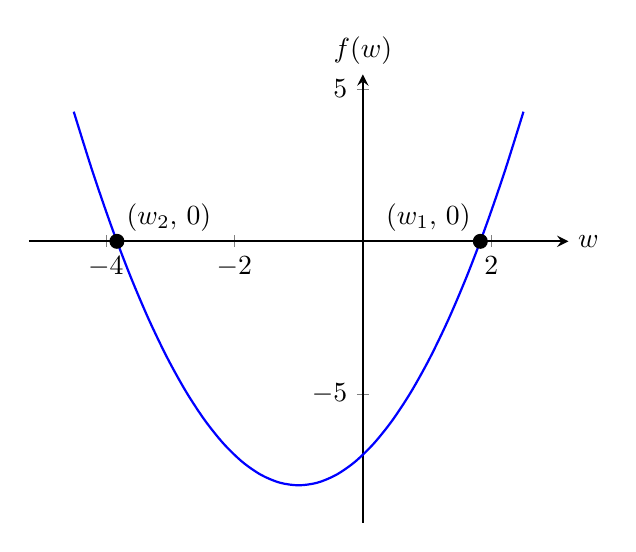
\begin{tikzpicture}
\tikzset{%%
  every mark/.append style={scale=1.0},%%
  scale=1.0%%
}
\pgfplotsset{%%
  every axis/.append style={font=\normalsize}%%
}
%%
\begin{axis}[%%
  axis line style=thick,%%
  axis lines=center,%%
  dotStyle/.style={only marks,mark size=2.5,black,mark color=black,mark=*},%%
  enlargelimits=true,%%
  plotStyle/.style={%%
    domain=-4.5:2.5,%%
    mark=none,%%
    smooth,%%
    thick%%
  },%%
  %%
  %% x-axis
  xlabel={\normalsize $w$},%%
  xlabel style=right,%%
  %%
  %% y-axis
  ylabel={\normalsize $f(w)$},%%
  ylabel style=above%%
]
%%
%%
%% The function f(x).
\addplot+ [plotStyle]
{x^2 + 2*x - 7};
%%
%% Some points on the graph of f(x).
\addplot[dotStyle] coordinates {
  (-2*sqrt(2)-1,0)
  (2*sqrt(2)-1,0)
};
%%
%% Label the above points.
\node[above right] at (axis cs:-3.82842712474619,0) {$\tuple{w_2}{0}$};
\node[above left] at (axis cs:1.82842712474619,0) {$\tuple{w_1}{0}$};
\end{axis}
\end{tikzpicture}

\end{document}
